
\documentclass[letterpaper,hide notes,xcolor={table,svgnames},pdftex,10pt]{beamer}
\def\showexamples{t}


%\usepackage[svgnames]{xcolor}

%% Demo talk
%\documentclass[letterpaper,notes=show]{beamer}

\usecolortheme{crane}
\setbeamertemplate{navigation symbols}{}

\usetheme{MyPittsburgh}
%\usetheme{Frankfurt}

%\usepackage{tipa}

\usepackage{hyperref}
\usepackage{graphicx,xspace}
\usepackage[normalem]{ulem}
\usepackage{multicol}

\newcommand\SF[1]{$\bigstar$\footnote{SF: #1}}

\usepackage[default]{sourcesanspro}
\usepackage[T1]{fontenc}

\newcounter{tmpnumSlide}
\newcounter{tmpnumNote}

% old question code
%\newcommand\question[1]{{$\bigstar$ \small \onlySlide{2}{#1}}}
% \newcommand\nquestion[1]{\ifdefined \presentationonly \textcircled{?} \fi \note{\par{\Large \textbf{?}} #1}}
% \newcommand\nanswer[1]{\note{\par{\Large \textbf{A}} #1}}


 \newcommand\mnote[1]{%
   \addtocounter{tmpnumSlide}{1}
   \ifdefined\showcues {~\tiny\fbox{\arabic{tmpnumSlide}}}\fi
   \note{\setlength{\parskip}{1ex}\addtocounter{tmpnumNote}{1}\textbf{\Large \arabic{tmpnumNote}:} {#1\par}}}

\newcommand\mmnote[1]{\note{\setlength{\parskip}{1ex}#1\par}}

%\newcommand\mnote[2][]{\ifdefined\handoutwithnotes {~\tiny\fbox{#1}}\fi
% \note{\setlength{\parskip}{1ex}\textbf{\Large #1:} #2\par}}

%\newcommand\mnote[2][]{{\tiny\fbox{#1}} \note{\setlength{\parskip}{1ex}\textbf{\Large #1:} #2\par}}

\newcommand\mquestion[2]{{~\color{red}\fbox{?}}\note{\setlength{\parskip}{1ex}\par{\Large \textbf{?}} #1} \note{\setlength{\parskip}{1ex}\par{\Large \textbf{A}} #2\par}\ifdefined \presentationonly \pause \fi}

\newcommand\blackboard[1]{%
\ifdefined   \showblackboard
  {#1}
  \else {\begin{center} \fbox{\colorbox{blue!30}{%
         \begin{minipage}{.95\linewidth}%
           \hspace{\stretch{1}} Some space intentionally left blank; done at the blackboard.%
         \end{minipage}}}\end{center}}%
         \fi%
}



%\newcommand\q{\tikz \node[thick,color=black,shape=circle]{?};}
%\newcommand\q{\ifdefined \presentationonly \textcircled{?} \fi}

\usepackage{listings}
\lstset{%
  keywordstyle=\bfseries,
  aboveskip=15pt,
  belowskip=15pt,
  captionpos=b,
  identifierstyle=\ttfamily,
  escapeinside={(*@}{@*)},
  stringstyle=\ttfamiliy,
  frame=lines,
  numbers=left, basicstyle=\scriptsize, numberstyle=\tiny, stepnumber=0, numbersep=2pt}

\usepackage{siunitx}
\newcommand\sius[1]{\num[group-separator = {,}]{#1}\si{\micro\second}}
\newcommand\sims[1]{\num[group-separator = {,}]{#1}\si{\milli\second}}
\newcommand\sins[1]{\num[group-separator = {,}]{#1}\si{\nano\second}}
\sisetup{group-separator = {,}, group-digits = true}

%% -------------------- tikz --------------------
\usepackage{tikz}
\usetikzlibrary{positioning}
\usetikzlibrary{arrows,backgrounds,automata,decorations.shapes,decorations.pathmorphing,decorations.markings,decorations.text}

\tikzstyle{place}=[circle,draw=blue!50,fill=blue!20,thick, inner sep=0pt,minimum size=6mm]
\tikzstyle{transition}=[rectangle,draw=black!50,fill=black!20,thick, inner sep=0pt,minimum size=4mm]

\tikzstyle{block}=[rectangle,draw=black, thick, inner sep=5pt]
\tikzstyle{bullet}=[circle,draw=black, fill=black, thin, inner sep=2pt]

\tikzstyle{pre}=[<-,shorten <=1pt,>=stealth',semithick]
\tikzstyle{post}=[->,shorten >=1pt,>=stealth',semithick]
\tikzstyle{bi}=[<->,shorten >=1pt,shorten <=1pt, >=stealth',semithick]

\tikzstyle{mut}=[-,>=stealth',semithick]

\tikzstyle{treereset}=[dashed,->, shorten >=1pt,>=stealth',thin]

\usepackage{ifmtarg}
\usepackage{xifthen}
\makeatletter
% new counter to now which frame it is within the sequence
\newcounter{multiframecounter}
% initialize buffer for previously used frame title
\gdef\lastframetitle{\textit{undefined}}
% new environment for a multi-frame
\newenvironment{multiframe}[1][]{%
\ifthenelse{\isempty{#1}}{%
% if no frame title was set via optional parameter,
% only increase sequence counter by 1
\addtocounter{multiframecounter}{1}%
}{%
% new frame title has been provided, thus
% reset sequence counter to 1 and buffer frame title for later use
\setcounter{multiframecounter}{1}%
\gdef\lastframetitle{#1}%
}%
% start conventional frame environment and
% automatically set frame title followed by sequence counter
\begin{frame}%
\frametitle{\lastframetitle~{\normalfont(\arabic{multiframecounter})}}%
}{%
\end{frame}%
}
\makeatother

\makeatletter
\newdimen\tu@tmpa%
\newdimen\ydiffl%
\newdimen\xdiffl%
\newcommand\ydiff[2]{%
    \coordinate (tmpnamea) at (#1);%
    \coordinate (tmpnameb) at (#2);%
    \pgfextracty{\tu@tmpa}{\pgfpointanchor{tmpnamea}{center}}%
    \pgfextracty{\ydiffl}{\pgfpointanchor{tmpnameb}{center}}%
    \advance\ydiffl by -\tu@tmpa%
}
\newcommand\xdiff[2]{%
    \coordinate (tmpnamea) at (#1);%
    \coordinate (tmpnameb) at (#2);%
    \pgfextractx{\tu@tmpa}{\pgfpointanchor{tmpnamea}{center}}%
    \pgfextractx{\xdiffl}{\pgfpointanchor{tmpnameb}{center}}%
    \advance\xdiffl by -\tu@tmpa%
}
\makeatother
\newcommand{\copyrightbox}[3][r]{%
\begin{tikzpicture}%
\node[inner sep=0pt,minimum size=2em](ciimage){#2};
\usefont{OT1}{phv}{n}{n}\fontsize{4}{4}\selectfont
\ydiff{ciimage.south}{ciimage.north}
\xdiff{ciimage.west}{ciimage.east}
\ifthenelse{\equal{#1}{r}}{%
\node[inner sep=0pt,right=1ex of ciimage.south east,anchor=north west,rotate=90]%
{\raggedleft\color{black!50}\parbox{\the\ydiffl}{\raggedright{}#3}};%
}{%
\ifthenelse{\equal{#1}{l}}{%
\node[inner sep=0pt,right=1ex of ciimage.south west,anchor=south west,rotate=90]%
{\raggedleft\color{black!50}\parbox{\the\ydiffl}{\raggedright{}#3}};%
}{%
\node[inner sep=0pt,below=1ex of ciimage.south west,anchor=north west]%
{\raggedleft\color{black!50}\parbox{\the\xdiffl}{\raggedright{}#3}};%
}
}
\end{tikzpicture}
}


%% --------------------

%\usepackage[excludeor]{everyhook}
%\PushPreHook{par}{\setbox0=\lastbox\llap{MUH}}\box0}

%\vspace*{\stretch{1}

%\setbox0=\lastbox \llap{\textbullet\enskip}\box0}

\setlength{\parskip}{\fill}

\newcommand\noskips{\setlength{\parskip}{1ex}}
\newcommand\doskips{\setlength{\parskip}{\fill}}

\newcommand\xx{\par\vspace*{\stretch{1}}\par}
\newcommand\xxs{\par\vspace*{2ex}\par}
\newcommand\tuple[1]{\langle #1 \rangle}
\newcommand\code[1]{{\sf \footnotesize #1}}
\newcommand\ex[1]{\uline{Example:} \ifdefined \presentationonly \pause \fi
  \ifdefined\showexamples#1\xspace\else{\uline{\hspace*{2cm}}}\fi}

\newcommand\ceil[1]{\lceil #1 \rceil}


\AtBeginSection[]
{
   \begin{frame}
       \frametitle{Outline}
       \tableofcontents[currentsection]
   \end{frame}
}



\pgfdeclarelayer{edgelayer}
\pgfdeclarelayer{nodelayer}
\pgfsetlayers{edgelayer,nodelayer,main}

\tikzstyle{none}=[inner sep=0pt]
\tikzstyle{rn}=[circle,fill=Red,draw=Black,line width=0.8 pt]
\tikzstyle{gn}=[circle,fill=Lime,draw=Black,line width=0.8 pt]
\tikzstyle{yn}=[circle,fill=Yellow,draw=Black,line width=0.8 pt]
\tikzstyle{empty}=[circle,fill=White,draw=Black]
\tikzstyle{bw} = [rectangle, draw, fill=blue!20, 
    text width=4em, text centered, rounded corners, minimum height=2em]
    
    \newcommand{\CcNote}[1]{% longname
	This work is licensed under the \textit{Creative Commons #1 3.0 License}.%
}
\newcommand{\CcImageBy}[1]{%
	\includegraphics[scale=#1]{creative_commons/cc_by_30.pdf}%
}
\newcommand{\CcImageSa}[1]{%
	\includegraphics[scale=#1]{creative_commons/cc_sa_30.pdf}%
}
\newcommand{\CcImageNc}[1]{%
	\includegraphics[scale=#1]{creative_commons/cc_nc_30.pdf}%
}
\newcommand{\CcGroupBySa}[2]{% zoom, gap
	\CcImageBy{#1}\hspace*{#2}\CcImageNc{#1}\hspace*{#2}\CcImageSa{#1}%
}
\newcommand{\CcLongnameByNcSa}{Attribution-NonCommercial-ShareAlike}

\newenvironment{changemargin}[1]{% 
  \begin{list}{}{% 
    \setlength{\topsep}{0pt}% 
    \setlength{\leftmargin}{#1}% 
    \setlength{\rightmargin}{1em}
    \setlength{\listparindent}{\parindent}% 
    \setlength{\itemindent}{\parindent}% 
    \setlength{\parsep}{\parskip}% 
  }% 
  \item[]}{\end{list}} 



\usepackage{multirow}

\title{Lecture 11 --- Use of Locks, Reentrancy}

\author{Jeff Zarnett \& Patrick Lam \\ \small \texttt{\{jzarnett, patrick.lam\}@uwaterloo.ca}}
\institute{Department of Electrical and Computer Engineering \\
  University of Waterloo}
\date{\today}


\begin{document}

\begin{frame}
  \titlepage

 \end{frame}


\part{Use of Locks}
\frame{\partpage}


\begin{frame}
\frametitle{Use of Locks}

\vspace*{-3em}
In previous courses: learned about locking and how it works.

Before: was enough to avoid bad stuff.

Now: Still important, but not enough.


\end{frame}


\begin{frame}
\frametitle{Critical Section Size}

  \begin{center}
    % Graphic for TeX using PGF
% Title: /home/plam/courses/p4p-2018/lectures/images/L07-critsec-size-1.dia
% Creator: Dia v0.97+git
% CreationDate: Thu Jan 25 10:13:37 2018
% For: plam
% \usepackage{tikz}
% The following commands are not supported in PSTricks at present
% We define them conditionally, so when they are implemented,
% this pgf file will use them.
\ifx\du\undefined
  \newlength{\du}
\fi
\setlength{\du}{15\unitlength}
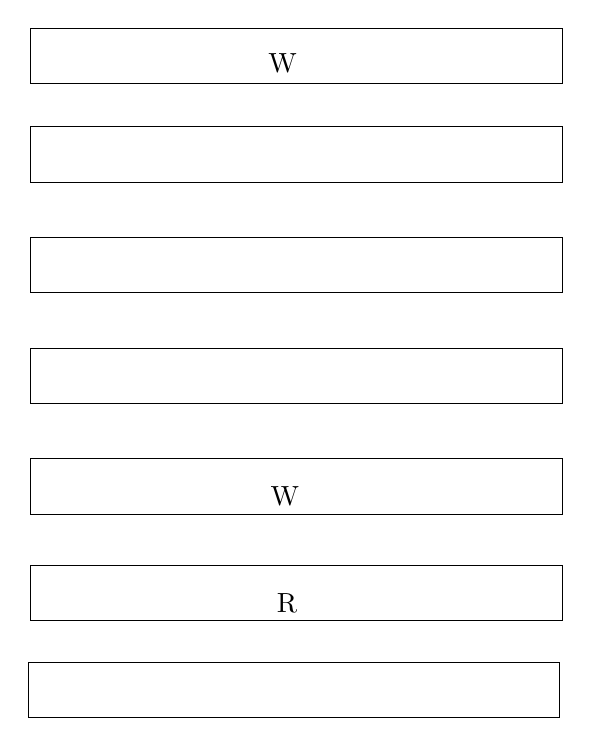
\begin{tikzpicture}[even odd rule]
\pgftransformxscale{1.000000}
\pgftransformyscale{-1.000000}
\definecolor{dialinecolor}{rgb}{0.000000, 0.000000, 0.000000}
\pgfsetstrokecolor{dialinecolor}
\pgfsetstrokeopacity{1.000000}
\definecolor{diafillcolor}{rgb}{1.000000, 1.000000, 1.000000}
\pgfsetfillcolor{diafillcolor}
\pgfsetfillopacity{1.000000}
\pgfsetlinewidth{0.100000\du}
\pgfsetdash{}{0pt}
\pgfsetmiterjoin
\pgfsetbuttcap
{\pgfsetcornersarced{\pgfpoint{0.000000\du}{0.000000\du}}\definecolor{diafillcolor}{rgb}{1.000000, 1.000000, 1.000000}
\pgfsetfillcolor{diafillcolor}
\pgfsetfillopacity{1.000000}
\fill (2.765000\du,2.100000\du)--(2.765000\du,2.800000\du)--(9.515000\du,2.800000\du)--(9.515000\du,2.100000\du)--cycle;
}{\pgfsetcornersarced{\pgfpoint{0.000000\du}{0.000000\du}}\definecolor{dialinecolor}{rgb}{0.000000, 0.000000, 0.000000}
\pgfsetstrokecolor{dialinecolor}
\pgfsetstrokeopacity{1.000000}
\draw (2.765000\du,2.100000\du)--(2.765000\du,2.800000\du)--(9.515000\du,2.800000\du)--(9.515000\du,2.100000\du)--cycle;
}\pgfsetlinewidth{0.100000\du}
\pgfsetdash{}{0pt}
\pgfsetmiterjoin
\pgfsetbuttcap
{\pgfsetcornersarced{\pgfpoint{0.000000\du}{0.000000\du}}\definecolor{diafillcolor}{rgb}{1.000000, 1.000000, 1.000000}
\pgfsetfillcolor{diafillcolor}
\pgfsetfillopacity{1.000000}
\fill (2.765000\du,3.355000\du)--(2.765000\du,4.055000\du)--(9.515000\du,4.055000\du)--(9.515000\du,3.355000\du)--cycle;
}{\pgfsetcornersarced{\pgfpoint{0.000000\du}{0.000000\du}}\definecolor{dialinecolor}{rgb}{0.000000, 0.000000, 0.000000}
\pgfsetstrokecolor{dialinecolor}
\pgfsetstrokeopacity{1.000000}
\draw (2.765000\du,3.355000\du)--(2.765000\du,4.055000\du)--(9.515000\du,4.055000\du)--(9.515000\du,3.355000\du)--cycle;
}\pgfsetlinewidth{0.100000\du}
\pgfsetdash{}{0pt}
\pgfsetmiterjoin
\pgfsetbuttcap
{\pgfsetcornersarced{\pgfpoint{0.000000\du}{0.000000\du}}\definecolor{diafillcolor}{rgb}{1.000000, 1.000000, 1.000000}
\pgfsetfillcolor{diafillcolor}
\pgfsetfillopacity{1.000000}
\fill (2.765000\du,4.760000\du)--(2.765000\du,5.460000\du)--(9.515000\du,5.460000\du)--(9.515000\du,4.760000\du)--cycle;
}{\pgfsetcornersarced{\pgfpoint{0.000000\du}{0.000000\du}}\definecolor{dialinecolor}{rgb}{0.000000, 0.000000, 0.000000}
\pgfsetstrokecolor{dialinecolor}
\pgfsetstrokeopacity{1.000000}
\draw (2.765000\du,4.760000\du)--(2.765000\du,5.460000\du)--(9.515000\du,5.460000\du)--(9.515000\du,4.760000\du)--cycle;
}\pgfsetlinewidth{0.100000\du}
\pgfsetdash{}{0pt}
\pgfsetmiterjoin
\pgfsetbuttcap
{\pgfsetcornersarced{\pgfpoint{0.000000\du}{0.000000\du}}\definecolor{diafillcolor}{rgb}{1.000000, 1.000000, 1.000000}
\pgfsetfillcolor{diafillcolor}
\pgfsetfillopacity{1.000000}
\fill (2.765000\du,6.165000\du)--(2.765000\du,6.865000\du)--(9.515000\du,6.865000\du)--(9.515000\du,6.165000\du)--cycle;
}{\pgfsetcornersarced{\pgfpoint{0.000000\du}{0.000000\du}}\definecolor{dialinecolor}{rgb}{0.000000, 0.000000, 0.000000}
\pgfsetstrokecolor{dialinecolor}
\pgfsetstrokeopacity{1.000000}
\draw (2.765000\du,6.165000\du)--(2.765000\du,6.865000\du)--(9.515000\du,6.865000\du)--(9.515000\du,6.165000\du)--cycle;
}\pgfsetlinewidth{0.100000\du}
\pgfsetdash{}{0pt}
\pgfsetmiterjoin
\pgfsetbuttcap
{\pgfsetcornersarced{\pgfpoint{0.000000\du}{0.000000\du}}\definecolor{diafillcolor}{rgb}{1.000000, 1.000000, 1.000000}
\pgfsetfillcolor{diafillcolor}
\pgfsetfillopacity{1.000000}
\fill (2.765000\du,7.570000\du)--(2.765000\du,8.270000\du)--(9.515000\du,8.270000\du)--(9.515000\du,7.570000\du)--cycle;
}{\pgfsetcornersarced{\pgfpoint{0.000000\du}{0.000000\du}}\definecolor{dialinecolor}{rgb}{0.000000, 0.000000, 0.000000}
\pgfsetstrokecolor{dialinecolor}
\pgfsetstrokeopacity{1.000000}
\draw (2.765000\du,7.570000\du)--(2.765000\du,8.270000\du)--(9.515000\du,8.270000\du)--(9.515000\du,7.570000\du)--cycle;
}\pgfsetlinewidth{0.100000\du}
\pgfsetdash{}{0pt}
\pgfsetmiterjoin
\pgfsetbuttcap
{\pgfsetcornersarced{\pgfpoint{0.000000\du}{0.000000\du}}\definecolor{diafillcolor}{rgb}{1.000000, 1.000000, 1.000000}
\pgfsetfillcolor{diafillcolor}
\pgfsetfillopacity{1.000000}
\fill (2.765000\du,8.925000\du)--(2.765000\du,9.625000\du)--(9.515000\du,9.625000\du)--(9.515000\du,8.925000\du)--cycle;
}{\pgfsetcornersarced{\pgfpoint{0.000000\du}{0.000000\du}}\definecolor{dialinecolor}{rgb}{0.000000, 0.000000, 0.000000}
\pgfsetstrokecolor{dialinecolor}
\pgfsetstrokeopacity{1.000000}
\draw (2.765000\du,8.925000\du)--(2.765000\du,9.625000\du)--(9.515000\du,9.625000\du)--(9.515000\du,8.925000\du)--cycle;
}% setfont left to latex
\definecolor{dialinecolor}{rgb}{0.000000, 0.000000, 0.000000}
\pgfsetstrokecolor{dialinecolor}
\pgfsetstrokeopacity{1.000000}
\definecolor{diafillcolor}{rgb}{0.000000, 0.000000, 0.000000}
\pgfsetfillcolor{diafillcolor}
\pgfsetfillopacity{1.000000}
\node[anchor=base west,inner sep=0pt,outer sep=0pt,color=dialinecolor] at (5.786450\du,2.662130\du){W};
% setfont left to latex
\definecolor{dialinecolor}{rgb}{0.000000, 0.000000, 0.000000}
\pgfsetstrokecolor{dialinecolor}
\pgfsetstrokeopacity{1.000000}
\definecolor{diafillcolor}{rgb}{0.000000, 0.000000, 0.000000}
\pgfsetfillcolor{diafillcolor}
\pgfsetfillopacity{1.000000}
\node[anchor=base west,inner sep=0pt,outer sep=0pt,color=dialinecolor] at (5.812130\du,8.169530\du){W};
% setfont left to latex
\definecolor{dialinecolor}{rgb}{0.000000, 0.000000, 0.000000}
\pgfsetstrokecolor{dialinecolor}
\pgfsetstrokeopacity{1.000000}
\definecolor{diafillcolor}{rgb}{0.000000, 0.000000, 0.000000}
\pgfsetfillcolor{diafillcolor}
\pgfsetfillopacity{1.000000}
\node[anchor=base west,inner sep=0pt,outer sep=0pt,color=dialinecolor] at (5.892510\du,9.522490\du){R};
\pgfsetlinewidth{0.100000\du}
\pgfsetdash{}{0pt}
\pgfsetmiterjoin
\pgfsetbuttcap
{\pgfsetcornersarced{\pgfpoint{0.000000\du}{0.000000\du}}\definecolor{diafillcolor}{rgb}{1.000000, 1.000000, 1.000000}
\pgfsetfillcolor{diafillcolor}
\pgfsetfillopacity{1.000000}
\fill (2.730000\du,10.155000\du)--(2.730000\du,10.855000\du)--(9.480000\du,10.855000\du)--(9.480000\du,10.155000\du)--cycle;
}{\pgfsetcornersarced{\pgfpoint{0.000000\du}{0.000000\du}}\definecolor{dialinecolor}{rgb}{0.000000, 0.000000, 0.000000}
\pgfsetstrokecolor{dialinecolor}
\pgfsetstrokeopacity{1.000000}
\draw (2.730000\du,10.155000\du)--(2.730000\du,10.855000\du)--(9.480000\du,10.855000\du)--(9.480000\du,10.155000\du)--cycle;
}\end{tikzpicture}

  \end{center}

\end{frame}

\begin{frame}
\frametitle{Critical Section Size}

  \begin{center}
    \input{images/L07-critsec-size-2}
  \end{center}

Critical sections should be as large as they need to be but no larger. 

\end{frame}


\begin{frame}
\frametitle{Rewrite This Block}

  \begin{center}
    % Graphic for TeX using PGF
% Title: /home/plam/courses/p4p-2018/lectures/images/L07-critsec-size-3.dia
% Creator: Dia v0.97+git
% CreationDate: Thu Jan 25 10:18:58 2018
% For: plam
% \usepackage{tikz}
% The following commands are not supported in PSTricks at present
% We define them conditionally, so when they are implemented,
% this pgf file will use them.
\ifx\du\undefined
  \newlength{\du}
\fi
\setlength{\du}{15\unitlength}
\begin{tikzpicture}[even odd rule]
\pgftransformxscale{1.000000}
\pgftransformyscale{-1.000000}
\definecolor{dialinecolor}{rgb}{0.000000, 0.000000, 0.000000}
\pgfsetstrokecolor{dialinecolor}
\pgfsetstrokeopacity{1.000000}
\definecolor{diafillcolor}{rgb}{1.000000, 1.000000, 1.000000}
\pgfsetfillcolor{diafillcolor}
\pgfsetfillopacity{1.000000}
\pgfsetlinewidth{0.100000\du}
\pgfsetdash{{\pgflinewidth}{0.200000\du}}{0cm}
\pgfsetmiterjoin
\pgfsetbuttcap
{\pgfsetcornersarced{\pgfpoint{0.000000\du}{0.000000\du}}\definecolor{diafillcolor}{rgb}{1.000000, 1.000000, 1.000000}
\pgfsetfillcolor{diafillcolor}
\pgfsetfillopacity{1.000000}
\fill (2.122464\du,1.675000\du)--(2.122464\du,9.875000\du)--(10.122464\du,9.875000\du)--(10.122464\du,1.675000\du)--cycle;
}{\pgfsetcornersarced{\pgfpoint{0.000000\du}{0.000000\du}}\definecolor{dialinecolor}{rgb}{0.000000, 0.000000, 0.000000}
\pgfsetstrokecolor{dialinecolor}
\pgfsetstrokeopacity{1.000000}
\draw (2.122464\du,1.675000\du)--(2.122464\du,9.875000\du)--(10.122464\du,9.875000\du)--(10.122464\du,1.675000\du)--cycle;
}\pgfsetlinewidth{0.100000\du}
\pgfsetdash{}{0pt}
\pgfsetmiterjoin
\pgfsetbuttcap
{\pgfsetcornersarced{\pgfpoint{0.000000\du}{0.000000\du}}\definecolor{diafillcolor}{rgb}{1.000000, 1.000000, 1.000000}
\pgfsetfillcolor{diafillcolor}
\pgfsetfillopacity{1.000000}
\fill (2.765000\du,2.100000\du)--(2.765000\du,2.800000\du)--(9.515000\du,2.800000\du)--(9.515000\du,2.100000\du)--cycle;
}{\pgfsetcornersarced{\pgfpoint{0.000000\du}{0.000000\du}}\definecolor{dialinecolor}{rgb}{0.000000, 0.000000, 0.000000}
\pgfsetstrokecolor{dialinecolor}
\pgfsetstrokeopacity{1.000000}
\draw (2.765000\du,2.100000\du)--(2.765000\du,2.800000\du)--(9.515000\du,2.800000\du)--(9.515000\du,2.100000\du)--cycle;
}\pgfsetlinewidth{0.100000\du}
\pgfsetdash{}{0pt}
\pgfsetmiterjoin
\pgfsetbuttcap
{\pgfsetcornersarced{\pgfpoint{0.000000\du}{0.000000\du}}\definecolor{diafillcolor}{rgb}{1.000000, 1.000000, 1.000000}
\pgfsetfillcolor{diafillcolor}
\pgfsetfillopacity{1.000000}
\fill (2.765000\du,3.355000\du)--(2.765000\du,4.055000\du)--(9.515000\du,4.055000\du)--(9.515000\du,3.355000\du)--cycle;
}{\pgfsetcornersarced{\pgfpoint{0.000000\du}{0.000000\du}}\definecolor{dialinecolor}{rgb}{0.000000, 0.000000, 0.000000}
\pgfsetstrokecolor{dialinecolor}
\pgfsetstrokeopacity{1.000000}
\draw (2.765000\du,3.355000\du)--(2.765000\du,4.055000\du)--(9.515000\du,4.055000\du)--(9.515000\du,3.355000\du)--cycle;
}\pgfsetlinewidth{0.100000\du}
\pgfsetdash{}{0pt}
\pgfsetmiterjoin
\pgfsetbuttcap
{\pgfsetcornersarced{\pgfpoint{0.000000\du}{0.000000\du}}\definecolor{diafillcolor}{rgb}{1.000000, 1.000000, 1.000000}
\pgfsetfillcolor{diafillcolor}
\pgfsetfillopacity{1.000000}
\fill (2.765000\du,4.760000\du)--(2.765000\du,5.460000\du)--(9.515000\du,5.460000\du)--(9.515000\du,4.760000\du)--cycle;
}{\pgfsetcornersarced{\pgfpoint{0.000000\du}{0.000000\du}}\definecolor{dialinecolor}{rgb}{0.000000, 0.000000, 0.000000}
\pgfsetstrokecolor{dialinecolor}
\pgfsetstrokeopacity{1.000000}
\draw (2.765000\du,4.760000\du)--(2.765000\du,5.460000\du)--(9.515000\du,5.460000\du)--(9.515000\du,4.760000\du)--cycle;
}\pgfsetlinewidth{0.100000\du}
\pgfsetdash{}{0pt}
\pgfsetmiterjoin
\pgfsetbuttcap
{\pgfsetcornersarced{\pgfpoint{0.000000\du}{0.000000\du}}\definecolor{diafillcolor}{rgb}{1.000000, 1.000000, 1.000000}
\pgfsetfillcolor{diafillcolor}
\pgfsetfillopacity{1.000000}
\fill (2.765000\du,6.165000\du)--(2.765000\du,6.865000\du)--(9.515000\du,6.865000\du)--(9.515000\du,6.165000\du)--cycle;
}{\pgfsetcornersarced{\pgfpoint{0.000000\du}{0.000000\du}}\definecolor{dialinecolor}{rgb}{0.000000, 0.000000, 0.000000}
\pgfsetstrokecolor{dialinecolor}
\pgfsetstrokeopacity{1.000000}
\draw (2.765000\du,6.165000\du)--(2.765000\du,6.865000\du)--(9.515000\du,6.865000\du)--(9.515000\du,6.165000\du)--cycle;
}\pgfsetlinewidth{0.100000\du}
\pgfsetdash{}{0pt}
\pgfsetmiterjoin
\pgfsetbuttcap
{\pgfsetcornersarced{\pgfpoint{0.000000\du}{0.000000\du}}\definecolor{diafillcolor}{rgb}{1.000000, 1.000000, 1.000000}
\pgfsetfillcolor{diafillcolor}
\pgfsetfillopacity{1.000000}
\fill (2.765000\du,7.570000\du)--(2.765000\du,8.270000\du)--(9.515000\du,8.270000\du)--(9.515000\du,7.570000\du)--cycle;
}{\pgfsetcornersarced{\pgfpoint{0.000000\du}{0.000000\du}}\definecolor{dialinecolor}{rgb}{0.000000, 0.000000, 0.000000}
\pgfsetstrokecolor{dialinecolor}
\pgfsetstrokeopacity{1.000000}
\draw (2.765000\du,7.570000\du)--(2.765000\du,8.270000\du)--(9.515000\du,8.270000\du)--(9.515000\du,7.570000\du)--cycle;
}\pgfsetlinewidth{0.100000\du}
\pgfsetdash{}{0pt}
\pgfsetmiterjoin
\pgfsetbuttcap
{\pgfsetcornersarced{\pgfpoint{0.000000\du}{0.000000\du}}\definecolor{diafillcolor}{rgb}{1.000000, 1.000000, 1.000000}
\pgfsetfillcolor{diafillcolor}
\pgfsetfillopacity{1.000000}
\fill (2.765000\du,8.925000\du)--(2.765000\du,9.625000\du)--(9.515000\du,9.625000\du)--(9.515000\du,8.925000\du)--cycle;
}{\pgfsetcornersarced{\pgfpoint{0.000000\du}{0.000000\du}}\definecolor{dialinecolor}{rgb}{0.000000, 0.000000, 0.000000}
\pgfsetstrokecolor{dialinecolor}
\pgfsetstrokeopacity{1.000000}
\draw (2.765000\du,8.925000\du)--(2.765000\du,9.625000\du)--(9.515000\du,9.625000\du)--(9.515000\du,8.925000\du)--cycle;
}% setfont left to latex
\definecolor{dialinecolor}{rgb}{0.000000, 0.000000, 0.000000}
\pgfsetstrokecolor{dialinecolor}
\pgfsetstrokeopacity{1.000000}
\definecolor{diafillcolor}{rgb}{0.000000, 0.000000, 0.000000}
\pgfsetfillcolor{diafillcolor}
\pgfsetfillopacity{1.000000}
\node[anchor=base west,inner sep=0pt,outer sep=0pt,color=dialinecolor] at (5.786447\du,2.662132\du){W};
% setfont left to latex
\definecolor{dialinecolor}{rgb}{0.000000, 0.000000, 0.000000}
\pgfsetstrokecolor{dialinecolor}
\pgfsetstrokeopacity{1.000000}
\definecolor{diafillcolor}{rgb}{0.000000, 0.000000, 0.000000}
\pgfsetfillcolor{diafillcolor}
\pgfsetfillopacity{1.000000}
\node[anchor=base west,inner sep=0pt,outer sep=0pt,color=dialinecolor] at (5.812128\du,8.169528\du){W};
% setfont left to latex
\definecolor{dialinecolor}{rgb}{0.000000, 0.000000, 0.000000}
\pgfsetstrokecolor{dialinecolor}
\pgfsetstrokeopacity{1.000000}
\definecolor{diafillcolor}{rgb}{0.000000, 0.000000, 0.000000}
\pgfsetfillcolor{diafillcolor}
\pgfsetfillopacity{1.000000}
\node[anchor=base west,inner sep=0pt,outer sep=0pt,color=dialinecolor] at (5.892513\du,9.522487\du){R};
\pgfsetlinewidth{0.100000\du}
\pgfsetdash{}{0pt}
\pgfsetmiterjoin
\pgfsetbuttcap
{\pgfsetcornersarced{\pgfpoint{0.000000\du}{0.000000\du}}\definecolor{diafillcolor}{rgb}{1.000000, 1.000000, 1.000000}
\pgfsetfillcolor{diafillcolor}
\pgfsetfillopacity{1.000000}
\fill (2.752464\du,10.280000\du)--(2.752464\du,10.980000\du)--(9.502464\du,10.980000\du)--(9.502464\du,10.280000\du)--cycle;
}{\pgfsetcornersarced{\pgfpoint{0.000000\du}{0.000000\du}}\definecolor{dialinecolor}{rgb}{0.000000, 0.000000, 0.000000}
\pgfsetstrokecolor{dialinecolor}
\pgfsetstrokeopacity{1.000000}
\draw (2.752464\du,10.280000\du)--(2.752464\du,10.980000\du)--(9.502464\du,10.980000\du)--(9.502464\du,10.280000\du)--cycle;
}% setfont left to latex
\definecolor{dialinecolor}{rgb}{0.000000, 0.000000, 0.000000}
\pgfsetstrokecolor{dialinecolor}
\pgfsetstrokeopacity{1.000000}
\definecolor{diafillcolor}{rgb}{0.000000, 0.000000, 0.000000}
\pgfsetfillcolor{diafillcolor}
\pgfsetfillopacity{1.000000}
\node[anchor=base west,inner sep=0pt,outer sep=0pt,color=dialinecolor] at (10.472464\du,2.225000\du){lock acquired};
\pgfsetlinewidth{0.100000\du}
\pgfsetdash{}{0pt}
\pgfsetbuttcap
{
\definecolor{diafillcolor}{rgb}{0.000000, 0.000000, 0.000000}
\pgfsetfillcolor{diafillcolor}
\pgfsetfillopacity{1.000000}
% was here!!!
\pgfsetarrowsstart{stealth}
\definecolor{dialinecolor}{rgb}{0.000000, 0.000000, 0.000000}
\pgfsetstrokecolor{dialinecolor}
\pgfsetstrokeopacity{1.000000}
\pgfpathmoveto{\pgfpoint{10.372484\du}{10.024981\du}}
\pgfpatharc{406}{287}{2.080465\du and 2.080465\du}
\pgfusepath{stroke}
}
% setfont left to latex
\definecolor{dialinecolor}{rgb}{0.000000, 0.000000, 0.000000}
\pgfsetstrokecolor{dialinecolor}
\pgfsetstrokeopacity{1.000000}
\definecolor{diafillcolor}{rgb}{0.000000, 0.000000, 0.000000}
\pgfsetfillcolor{diafillcolor}
\pgfsetfillopacity{1.000000}
\node[anchor=base west,inner sep=0pt,outer sep=0pt,color=dialinecolor] at (11.372464\du,7.625000\du){move outside lock};
\end{tikzpicture}

  \end{center}

Sometimes control flow or other very short statements might get swept into the critical section.

Those should be the exception rather than the rule.

\end{frame}


\begin{frame}[fragile]
\frametitle{Remember the Producer-Consumer Problem?}

Short code example from the producer-consumer problem:
\begin{lstlisting}[language=Rust]
for _j in 0 .. NUM_THREADS {
  // create consumers
  let spaces = spaces.clone();
  let items = items.clone();
  let buffer = buffer.clone();
  threads.push(
    thread::spawn(move || {
      for _k in 0 .. ITEMS_PER_THREAD {
        let permit = block_on(items.acquire());
        let mut buf = buffer.lock().unwrap();
        let current_consume_space = buf.consumer_count;
        let next_consume_space = (current_consume_space+1) % buf.buffer.len();
        let to_consume = *buf.buffer.get(current_consume_space).unwrap();
        buf.consumer_count = next_consume_space;
        spaces.add_permits(1);
        permit.forget();
        consume_item(to_consume);
      }
    })
  );
}

\end{lstlisting}

\end{frame}


\begin{frame}
\frametitle{Previously, More Explicit}

When we used locks in C (or similar), it was easier to identify what's in the critical section, because we had explicit lock and unlock statements. 

The explicit unlock statement, especially, made it much clearer where it ends. 

Now, we don't consider the critical section over until the \texttt{MutexGuard} (returned by \texttt{lock()}) goes out of scope. 

And that happens here at the end of the iteration of the loop.



\end{frame}




\begin{frame}
\frametitle{``Do you think you got him?''}

What I always say is to analyze this closure one statement at a time and look into which of these access shared variables. 

\begin{center}
	\includegraphics[width=\textwidth]{images/gothim.png}
\end{center}

\end{frame}


\begin{frame}
\frametitle{Better to be Safe than Sorry}

In a practical sense, the critical section needs to enclose anything that references \texttt{buf}.

Looking at that code, how did we do?

Rust is good about not letting you access shared data in an uncontrolled way.

But not so good at making sure nothing extra is there.

\end{frame}


\begin{frame}[fragile]
\frametitle{Option 1: Manual Scoping}

\begin{lstlisting}[language=Rust]
for _j in 0 .. NUM_THREADS {
 // create consumers
 let spaces = spaces.clone();
 let items = items.clone();
 let buffer = buffer.clone();
 threads.push(
   thread::spawn(move || {
     for _k in 0 .. ITEMS_PER_THREAD {
       let permit = block_on(items.acquire());
       let to_consume = {
         let mut buf = buffer.lock().unwrap();
         let current_consume_space = buf.consumer_count;
         let next_consume_space = (current_consume_space+1)%buf.buffer.len();
         let to_consume = *buf.buffer.get(current_consume_space).unwrap();
         buf.consumer_count = next_consume_space;
         to_consume
       };
       spaces.add_permits(1);
       permit.forget();
       consume_item(to_consume);
     }
   })
 );
}
\end{lstlisting}

\end{frame}

\begin{frame}
\frametitle{Option 2: Taking Out the Guard}

The other approach to making the \texttt{MutexGuard} go out of scope is to actually call \texttt{drop()} on it. 

\begin{center}
	\includegraphics[width=0.4\textwidth]{images/batty2.jpg}
\end{center}

This is effective in telling the compiler that it is time for this value to die. 

Calling \texttt{drop()} moves ownership of the MutexGuard to the \texttt{drop} function where it will go out of scope and be removed. 

\end{frame}


\begin{frame}
\frametitle{Like for Like}
I applied a similar change to the producer code as we just discussed about the consumer. 
 
I added some thread sleeps to the original and modified program so it appears that consuming or producing an item actually takes meaningful work. 

Benchmarks are created with \texttt{hyperfine --warmup 1 -m 5 "cargo run --release"}.
 

\end{frame}


\begin{frame}
\frametitle{Test Results}

Unoptimized version: 2.8 seconds


Optimized version: 1.1 seconds


\end{frame}




\begin{frame}
\frametitle{Locks Have Costs}

Keeping the critical section as small as possible is important because it speeds up performance (reduces the serial portion of your program). 

But that's not the only reason. 

The lock is a resource, and contention for that resource is itself expensive.


\end{frame}


\begin{frame}
\frametitle{Locking Granularity}
Alright, we already know that locks prevent data races.

So we need to use them to prevent data races, but it's not as simple as it sounds. 

We have choices about the granularity of locking, and it is a trade-off.


  \begin{center}
    \includegraphics[scale=0.5]{images/lock-all-the-things}
  \end{center}
\end{frame}
%%%%%%%%%%%%%%%%%%%%%%%%%%%%%%%%%%%%%%%%%%%%%%%%%%%%%%%%%%%%%%%%%%%%%%%%%%%%%%%%

\begin{frame}
\frametitle{Coarse-Grained Lock}

  \begin{center}
    \input{images/L07-fine-grained-1}
  \end{center}

\end{frame}

\begin{frame}
\frametitle{Fine-Grained Locks}

  \begin{center}
    % Graphic for TeX using PGF
% Title: /home/plam/courses/p4p-2018/lectures/images/L07-fine-grained-2.dia
% Creator: Dia v0.97+git
% CreationDate: Thu Jan 25 10:28:49 2018
% For: plam
% \usepackage{tikz}
% The following commands are not supported in PSTricks at present
% We define them conditionally, so when they are implemented,
% this pgf file will use them.
\ifx\du\undefined
  \newlength{\du}
\fi
\setlength{\du}{15\unitlength}
\begin{tikzpicture}[even odd rule]
\pgftransformxscale{1.000000}
\pgftransformyscale{-1.000000}
\definecolor{dialinecolor}{rgb}{0.000000, 0.000000, 0.000000}
\pgfsetstrokecolor{dialinecolor}
\pgfsetstrokeopacity{1.000000}
\definecolor{diafillcolor}{rgb}{1.000000, 1.000000, 1.000000}
\pgfsetfillcolor{diafillcolor}
\pgfsetfillopacity{1.000000}
\pgfsetlinewidth{0.100000\du}
\pgfsetdash{{\pgflinewidth}{0.200000\du}}{0cm}
\pgfsetmiterjoin
\pgfsetbuttcap
{\pgfsetcornersarced{\pgfpoint{0.000000\du}{0.000000\du}}\definecolor{diafillcolor}{rgb}{1.000000, 1.000000, 1.000000}
\pgfsetfillcolor{diafillcolor}
\pgfsetfillopacity{1.000000}
\fill (4.750000\du,2.550000\du)--(4.750000\du,9.400000\du)--(7.700000\du,9.400000\du)--(7.700000\du,2.550000\du)--cycle;
}{\pgfsetcornersarced{\pgfpoint{0.000000\du}{0.000000\du}}\definecolor{dialinecolor}{rgb}{0.000000, 0.000000, 0.000000}
\pgfsetstrokecolor{dialinecolor}
\pgfsetstrokeopacity{1.000000}
\draw (4.750000\du,2.550000\du)--(4.750000\du,9.400000\du)--(7.700000\du,9.400000\du)--(7.700000\du,2.550000\du)--cycle;
}\pgfsetlinewidth{0.100000\du}
\pgfsetdash{{\pgflinewidth}{0.200000\du}}{0cm}
\pgfsetmiterjoin
\pgfsetbuttcap
{\pgfsetcornersarced{\pgfpoint{0.000000\du}{0.000000\du}}\definecolor{diafillcolor}{rgb}{1.000000, 1.000000, 1.000000}
\pgfsetfillcolor{diafillcolor}
\pgfsetfillopacity{1.000000}
\fill (1.100000\du,2.550000\du)--(1.100000\du,9.400000\du)--(4.350000\du,9.400000\du)--(4.350000\du,2.550000\du)--cycle;
}{\pgfsetcornersarced{\pgfpoint{0.000000\du}{0.000000\du}}\definecolor{dialinecolor}{rgb}{0.000000, 0.000000, 0.000000}
\pgfsetstrokecolor{dialinecolor}
\pgfsetstrokeopacity{1.000000}
\draw (1.100000\du,2.550000\du)--(1.100000\du,9.400000\du)--(4.350000\du,9.400000\du)--(4.350000\du,2.550000\du)--cycle;
}\pgfsetlinewidth{0.100000\du}
\pgfsetdash{}{0pt}
\pgfsetmiterjoin
\pgfsetbuttcap
{\pgfsetcornersarced{\pgfpoint{0.000000\du}{0.000000\du}}\definecolor{diafillcolor}{rgb}{1.000000, 1.000000, 1.000000}
\pgfsetfillcolor{diafillcolor}
\pgfsetfillopacity{1.000000}
\fill (1.980000\du,3.327500\du)--(1.980000\du,5.327500\du)--(4.030000\du,5.327500\du)--(4.030000\du,3.327500\du)--cycle;
}{\pgfsetcornersarced{\pgfpoint{0.000000\du}{0.000000\du}}\definecolor{dialinecolor}{rgb}{0.000000, 0.000000, 0.000000}
\pgfsetstrokecolor{dialinecolor}
\pgfsetstrokeopacity{1.000000}
\draw (1.980000\du,3.327500\du)--(1.980000\du,5.327500\du)--(4.030000\du,5.327500\du)--(4.030000\du,3.327500\du)--cycle;
}\pgfsetlinewidth{0.100000\du}
\pgfsetdash{}{0pt}
\pgfsetmiterjoin
\pgfsetbuttcap
{\pgfsetcornersarced{\pgfpoint{0.000000\du}{0.000000\du}}\definecolor{diafillcolor}{rgb}{1.000000, 1.000000, 1.000000}
\pgfsetfillcolor{diafillcolor}
\pgfsetfillopacity{1.000000}
\fill (5.035000\du,3.327500\du)--(5.035000\du,5.327500\du)--(7.085000\du,5.327500\du)--(7.085000\du,3.327500\du)--cycle;
}{\pgfsetcornersarced{\pgfpoint{0.000000\du}{0.000000\du}}\definecolor{dialinecolor}{rgb}{0.000000, 0.000000, 0.000000}
\pgfsetstrokecolor{dialinecolor}
\pgfsetstrokeopacity{1.000000}
\draw (5.035000\du,3.327500\du)--(5.035000\du,5.327500\du)--(7.085000\du,5.327500\du)--(7.085000\du,3.327500\du)--cycle;
}\pgfsetlinewidth{0.100000\du}
\pgfsetdash{}{0pt}
\pgfsetmiterjoin
\pgfsetbuttcap
{\pgfsetcornersarced{\pgfpoint{0.000000\du}{0.000000\du}}\definecolor{diafillcolor}{rgb}{1.000000, 1.000000, 1.000000}
\pgfsetfillcolor{diafillcolor}
\pgfsetfillopacity{1.000000}
\fill (1.980000\du,6.337500\du)--(1.980000\du,8.337500\du)--(4.030000\du,8.337500\du)--(4.030000\du,6.337500\du)--cycle;
}{\pgfsetcornersarced{\pgfpoint{0.000000\du}{0.000000\du}}\definecolor{dialinecolor}{rgb}{0.000000, 0.000000, 0.000000}
\pgfsetstrokecolor{dialinecolor}
\pgfsetstrokeopacity{1.000000}
\draw (1.980000\du,6.337500\du)--(1.980000\du,8.337500\du)--(4.030000\du,8.337500\du)--(4.030000\du,6.337500\du)--cycle;
}\pgfsetlinewidth{0.100000\du}
\pgfsetdash{}{0pt}
\pgfsetmiterjoin
\pgfsetbuttcap
{\pgfsetcornersarced{\pgfpoint{0.000000\du}{0.000000\du}}\definecolor{diafillcolor}{rgb}{1.000000, 1.000000, 1.000000}
\pgfsetfillcolor{diafillcolor}
\pgfsetfillopacity{1.000000}
\fill (5.035000\du,6.337500\du)--(5.035000\du,8.337500\du)--(7.085000\du,8.337500\du)--(7.085000\du,6.337500\du)--cycle;
}{\pgfsetcornersarced{\pgfpoint{0.000000\du}{0.000000\du}}\definecolor{dialinecolor}{rgb}{0.000000, 0.000000, 0.000000}
\pgfsetstrokecolor{dialinecolor}
\pgfsetstrokeopacity{1.000000}
\draw (5.035000\du,6.337500\du)--(5.035000\du,8.337500\du)--(7.085000\du,8.337500\du)--(7.085000\du,6.337500\du)--cycle;
}\pgfsetlinewidth{0.100000\du}
\pgfsetdash{}{0pt}
\pgfsetbuttcap
{
\definecolor{diafillcolor}{rgb}{0.000000, 0.000000, 0.000000}
\pgfsetfillcolor{diafillcolor}
\pgfsetfillopacity{1.000000}
% was here!!!
\pgfsetarrowsend{stealth}
\definecolor{dialinecolor}{rgb}{0.000000, 0.000000, 0.000000}
\pgfsetstrokecolor{dialinecolor}
\pgfsetstrokeopacity{1.000000}
\draw (2.600000\du,13.350000\du)--(2.934278\du,8.387412\du);
}
% setfont left to latex
\definecolor{dialinecolor}{rgb}{0.000000, 0.000000, 0.000000}
\pgfsetstrokecolor{dialinecolor}
\pgfsetstrokeopacity{1.000000}
\definecolor{diafillcolor}{rgb}{0.000000, 0.000000, 0.000000}
\pgfsetfillcolor{diafillcolor}
\pgfsetfillopacity{1.000000}
\node[anchor=base west,inner sep=0pt,outer sep=0pt,color=dialinecolor] at (3.400000\du,11.950000\du){thread 1};
\pgfsetlinewidth{0.100000\du}
\pgfsetdash{}{0pt}
\pgfsetbuttcap
{
\definecolor{diafillcolor}{rgb}{0.000000, 0.000000, 0.000000}
\pgfsetfillcolor{diafillcolor}
\pgfsetfillopacity{1.000000}
% was here!!!
\pgfsetarrowsend{stealth}
\definecolor{dialinecolor}{rgb}{0.000000, 0.000000, 0.000000}
\pgfsetstrokecolor{dialinecolor}
\pgfsetstrokeopacity{1.000000}
\draw (14.050000\du,3.450000\du)--(7.085000\du,4.327500\du);
}
% setfont left to latex
\definecolor{dialinecolor}{rgb}{0.000000, 0.000000, 0.000000}
\pgfsetstrokecolor{dialinecolor}
\pgfsetstrokeopacity{1.000000}
\definecolor{diafillcolor}{rgb}{0.000000, 0.000000, 0.000000}
\pgfsetfillcolor{diafillcolor}
\pgfsetfillopacity{1.000000}
\node[anchor=base west,inner sep=0pt,outer sep=0pt,color=dialinecolor] at (12.100000\du,4.450000\du){thread 2};
\pgfsetlinewidth{0.100000\du}
\pgfsetdash{}{0pt}
\pgfsetbuttcap
\pgfsetmiterjoin
\pgfsetlinewidth{0.100000\du}
\pgfsetbuttcap
\pgfsetmiterjoin
\pgfsetdash{}{0pt}
\definecolor{diafillcolor}{rgb}{1.000000, 0.000000, 0.000000}
\pgfsetfillcolor{diafillcolor}
\pgfsetfillopacity{1.000000}
\fill (8.587143\du,6.905000\du)--(9.122857\du,6.905000\du)--(9.480000\du,7.262143\du)--(9.480000\du,7.797857\du)--(9.122857\du,8.155000\du)--(8.587143\du,8.155000\du)--(8.230000\du,7.797857\du)--(8.230000\du,7.262143\du)--cycle;
\definecolor{dialinecolor}{rgb}{1.000000, 1.000000, 1.000000}
\pgfsetstrokecolor{dialinecolor}
\pgfsetstrokeopacity{1.000000}
\draw (8.587143\du,6.905000\du)--(9.122857\du,6.905000\du)--(9.480000\du,7.262143\du)--(9.480000\du,7.797857\du)--(9.122857\du,8.155000\du)--(8.587143\du,8.155000\du)--(8.230000\du,7.797857\du)--(8.230000\du,7.262143\du)--cycle;
\pgfsetlinewidth{0.100000\du}
\pgfsetdash{}{0pt}
\pgfsetbuttcap
{
\definecolor{diafillcolor}{rgb}{0.000000, 0.000000, 0.000000}
\pgfsetfillcolor{diafillcolor}
\pgfsetfillopacity{1.000000}
% was here!!!
\pgfsetarrowsend{stealth}
\definecolor{dialinecolor}{rgb}{0.000000, 0.000000, 0.000000}
\pgfsetstrokecolor{dialinecolor}
\pgfsetstrokeopacity{1.000000}
\draw (14.550000\du,8.400000\du)--(9.750000\du,7.650000\du);
}
% setfont left to latex
\definecolor{dialinecolor}{rgb}{0.000000, 0.000000, 0.000000}
\pgfsetstrokecolor{dialinecolor}
\pgfsetstrokeopacity{1.000000}
\definecolor{diafillcolor}{rgb}{0.000000, 0.000000, 0.000000}
\pgfsetfillcolor{diafillcolor}
\pgfsetfillopacity{1.000000}
\node[anchor=base west,inner sep=0pt,outer sep=0pt,color=dialinecolor] at (11.444564\du,7.650000\du){thread 3};
% setfont left to latex
\definecolor{dialinecolor}{rgb}{0.000000, 0.000000, 0.000000}
\pgfsetstrokecolor{dialinecolor}
\pgfsetstrokeopacity{1.000000}
\definecolor{diafillcolor}{rgb}{0.000000, 0.000000, 0.000000}
\pgfsetfillcolor{diafillcolor}
\pgfsetfillopacity{1.000000}
\node[anchor=base west,inner sep=0pt,outer sep=0pt,color=dialinecolor] at (1.150000\du,2.100000\du){lock 1};
% setfont left to latex
\definecolor{dialinecolor}{rgb}{0.000000, 0.000000, 0.000000}
\pgfsetstrokecolor{dialinecolor}
\pgfsetstrokeopacity{1.000000}
\definecolor{diafillcolor}{rgb}{0.000000, 0.000000, 0.000000}
\pgfsetfillcolor{diafillcolor}
\pgfsetfillopacity{1.000000}
\node[anchor=base west,inner sep=0pt,outer sep=0pt,color=dialinecolor] at (5.200000\du,2.150000\du){lock 2};
\end{tikzpicture}

  \end{center}

\end{frame}

\begin{frame}
\frametitle{Coarse-Grained vs Fine-Grained Locking}

\alert{Coarse-grained} locking is easier to write and harder to mess up, but it can significantly reduce opportunities for parallelism. 

\alert{Fine-grained locking} requires more careful design,
increases locking overhead and is more prone to bugs (deadlock etc).  


Locks' extents constitute their granularity. 

\end{frame}


\begin{frame}
\frametitle{Lock Concerns}

We'll discuss three major concerns when using locks:
  \begin{itemize}
    \item overhead;
    \item contention; and
    \item deadlocks.
  \end{itemize}
  
  
We aren't even talking about under-locking (i.e., remaining race conditions).

\end{frame}

\begin{frame}
\frametitle{Lock Overhead}

  Using a lock isn't free. You pay:
  \begin{itemize}
    \item allocated memory for the locks;
    \item initialization and destruction time; and
    \item acquisition and release time.
  \end{itemize}


  These costs scale with the number of locks that you have.
\end{frame}


\begin{frame}
\frametitle{Lock Contention}

\vspace*{-3em}
 Most locking time is wasted waiting for the lock to become available.\\[1em]
We can fix this by:
\vspace*{-3em}
      \begin{itemize}
        \item making the locking regions smaller (more granular); or
        \item making more locks for independent sections.
      \end{itemize}


\end{frame}

\begin{frame}
\frametitle{Deadlocks}

Finally, the more locks you have, the more you have to worry about deadlocks.

\begin{center}
	\includegraphics[width=0.5\textwidth]{images/deadlock.jpg}
\end{center}

As you know, the key condition for a deadlock is waiting for a lock held by process $X$ while holding a lock held by process $X'$. ($X = X'$ is allowed).

\end{frame}


\begin{frame}
\frametitle{Deadlocks}



Okay, in a formal sense, the four conditions for deadlock are:

\begin{enumerate}
	\item \textbf{Mutual Exclusion}
	\item \textbf{Hold-and-Wait}
	\item \textbf{No Preemption}
	\item \textbf{Circular-Wait}
\end{enumerate}

\end{frame}


\begin{frame}[fragile]
\frametitle{Simple Deadlock Example}

Consider, for instance, two processors trying to get two locks.

\begin{center}
  \begin{tabular}{ll}
\begin{minipage}{.4\textwidth}
      {\bf Thread 1}

      \verb+Get Lock 1+

      \verb+Get Lock 2+

      \verb+Release Lock 2+

      \verb+Release Lock 1+
\end{minipage} & 
\begin{minipage}{.4\textwidth}
      {\bf Thread 2}

      \verb+Get Lock 2+

      \verb+Get Lock 1+

      \verb+Release Lock 1+

      \verb+Release Lock 2+
\end{minipage}
\end{tabular}
\end{center}


\end{frame}

\begin{frame}[fragile]
\frametitle{Avoiding Deadlocks}

To avoid deadlocks, always be careful if your code {\bf acquires a lock while holding one}.  
  
You have two choices: (1) ensure consistent ordering in acquiring locks; or (2) use trylock.

As an example of consistent ordering:
\begin{center}
\begin{tabular}{ll}
\begin{minipage}{.4\textwidth}
  \begin{lstlisting}[language=Rust]
let mut thing1 = l1.lock().unwrap()
let mut thing2 = l2.lock().unwrap()
// protected code
// locks dropped when going out of scope
\end{lstlisting}
\end{minipage}&
\begin{minipage}{.4\textwidth}
\begin{lstlisting}[language=Rust]
let mut thing1 = l1.lock().unwrap()
let mut thing2 = l2.lock().unwrap()
// protected code
// locks dropped when going out of scope
  \end{lstlisting}
\end{minipage}
\end{tabular}
\end{center}

\end{frame}



\begin{frame}[fragile]
\frametitle{Trylock}

Alternately, you can use trylock. 

Recall that Pthreads' {\tt trylock} returns 0 if it gets the lock. 

But if it doesn't, your thread doesn't get blocked. 

  \begin{lstlisting}[language=Rust]
    loop {
        let mut m1 = l1.lock().unwrap();
        let m2 = l2.try_lock();
        if m2.is_ok() {
            *m1 += amount;
            *m2.unwrap() -= amount;
            break;
        } else {
            println!("try_lock failed");
            // Go around the loop again and try again
        }
    }
  \end{lstlisting}
  
This prevents the hold and wait condition.

\end{frame}



\begin{frame}
\frametitle{There Can Be Only One}

\begin{center}
	\includegraphics[width=0.8\textwidth]{images/giantlock.jpg}\\
	\hfill Photo Credit: Craig Middleton\footnote{\url{https://www.flickr.com/photos/craigmiddleton/3579668458}}
\end{center}


\end{frame}


\begin{frame}
\frametitle{Coarse-Grained Locking}

One way of avoiding problems due to locking is to use few locks
(1?). 

This is \emph{coarse-grained locking}; it does have a couple of advantages:
  \begin{itemize}
    \item it is easier to implement;
    \item with one lock, there is no chance of deadlocking; and
    \item it has the lowest memory usage and setup time possible.
  \end{itemize}

Your parallel program will quickly become sequential.


\end{frame}

\begin{frame}
\frametitle{Python}

Python puts a lock around the whole interpreter (known as the
\emph{global interpreter lock}).  

This is the main reason (most) scripting languages have poor parallel performance; Python's just an example.

Two major implications:
\begin{itemize}
\item The only performance benefit you'll see from threading is if one of the threads is
      waiting for I/O.
\item But: any non-I/O-bound threaded program will be {\bf slower} than the sequential
      version (plus, the interpreter will slow down your system).
\end{itemize}


\end{frame}

\begin{frame}
\frametitle{Fine-Grained Locking}

On the other end of the spectrum is \emph{fine-grained locking}. 


\begin{center}
	\includegraphics[width=0.4\textwidth]{images/tinylocks.jpeg}
\end{center}


\end{frame}

\begin{frame}
\frametitle{Fine-Grained Locking} 

The big advantage: it maximizes parallelization in your program.

However, it also comes with a number of disadvantages:
  \begin{itemize}
    \item if your program isn't very parallel, it'll be mostly wasted memory and setup time;
    \item plus, you're now prone to deadlocks; and
    \item fine-grained locking is generally more error-prone (be sure you grab the right lock!)
  \end{itemize}

\end{frame}

\begin{frame}
\frametitle{Lock Scope Examples}


    Databases may lock fields / records / tables. (fine-grained $\rightarrow$ coarse-grained).

    You can also lock individual objects (but beware: sometimes you need transactional guarantees.)



\end{frame}

\part{Reentrancy}
\frame{\partpage}


\begin{frame}
\frametitle{Out and In Again}

\begin{center}
	\includegraphics[width=0.5\textwidth]{images/revolvingdoor.jpg}
\end{center}

\end{frame}


\begin{frame}[fragile]
\frametitle{Non-Reentrant C Function}

The trivial example of a non-reentrant C function:

\begin{lstlisting}[language=C]
int tmp;

void swap( int x, int y ) {
    tmp = y;
    y = x;
    x = tmp;
}
\end{lstlisting}

Why is this non-reentrant?

How can we make it reentrant?

\end{frame}

%%%%%%%%%%%%%%%%%%%%%%%%%%%%%%%%%%%%%%%%%%%%%%%%%%%%%%%%%%%%%%%%%%%%%%%%%%%%%%%%
\begin{frame}
  \frametitle{Reentrancy}

  
    $\Rightarrow$ A function can be suspended in the middle and \\ {\bf re-entered}
      (called again) before the previous execution returns.\\[1em]
    
     Does not always mean {\bf thread-safe} (although it usually is).
      \begin{itemize}
        \item Recall: {\bf thread-safe} is essentially ``no data races''.
      \end{itemize}
 ~\\[1em]
  Moot point if the function only modifies local data, e.g. {\tt sin()}.
  
\end{frame}
%%%%%%%%%%%%%%%%%%%%%%%%%%%%%%%%%%%%%%%%%%%%%%%%%%%%%%%%%%%%%%%%%%%%%%%%%%%%%%%%

%%%%%%%%%%%%%%%%%%%%%%%%%%%%%%%%%%%%%%%%%%%%%%%%%%%%%%%%%%%%%%%%%%%%%%%%%%%%%%%%
\begin{frame}[fragile]
  \frametitle{Reentrancy Example}

  

  Courtesy of Wikipedia (with modifications):
  \begin{lstlisting}[language=C]
int t;
 
void swap(int *x, int *y) {
    t = *x;
    *x = *y;
    // hardware interrupt might invoke isr() here!
    *y = t;
}
 
void isr() {
    int x = 1, y = 2;
    swap(&x, &y);
}
...
int a = 3, b = 4;
...
    swap(&a, &b);
  \end{lstlisting}
  
\end{frame}
%%%%%%%%%%%%%%%%%%%%%%%%%%%%%%%%%%%%%%%%%%%%%%%%%%%%%%%%%%%%%%%%%%%%%%%%%%%%%%%%

%%%%%%%%%%%%%%%%%%%%%%%%%%%%%%%%%%%%%%%%%%%%%%%%%%%%%%%%%%%%%%%%%%%%%%%%%%%%%%%%
\begin{frame}[fragile]
  \frametitle{Reentrancy Example---Explained (a trace)}

  
  \begin{lstlisting}[language=C]
call swap(&a, &b);
 t = *x;                // t = 3 (a)
 *x = *y;               // a = 4 (b)
 call isr();
    x = 1; y = 2;
    call swap(&x, &y)
    t = *x;             // t = 1 (x)
    *x = *y;            // x = 2 (y)
    *y = t;             // y = 1
 *y = t;                // b = 1

Final values:
a = 4, b = 1

Expected values:
a = 4, b = 3
  \end{lstlisting}
  
\end{frame}
%%%%%%%%%%%%%%%%%%%%%%%%%%%%%%%%%%%%%%%%%%%%%%%%%%%%%%%%%%%%%%%%%%%%%%%%%%%%%%%%

%%%%%%%%%%%%%%%%%%%%%%%%%%%%%%%%%%%%%%%%%%%%%%%%%%%%%%%%%%%%%%%%%%%%%%%%%%%%%%%%
\begin{frame}[fragile]
  \frametitle{Reentrancy Example, Fixed}

  
  \begin{lstlisting}[language=C,escapechar=@]
int t;
 
void swap(int *x, int *y) {
    int s;
 
    @\alert{s = t}@;  // save global variable
    t = *x;
    *x = *y;
    // hardware interrupt might invoke isr() here!
    *y = t;
    @\alert{t = s}@;  // restore global variable
}
 
void isr() {
    int x = 1, y = 2;
    swap(&x, &y);
}
...
int a = 3, b = 4;
...
    swap(&a, &b);
  \end{lstlisting}
  
\end{frame}
%%%%%%%%%%%%%%%%%%%%%%%%%%%%%%%%%%%%%%%%%%%%%%%%%%%%%%%%%%%%%%%%%%%%%%%%%%%%%%%%

%%%%%%%%%%%%%%%%%%%%%%%%%%%%%%%%%%%%%%%%%%%%%%%%%%%%%%%%%%%%%%%%%%%%%%%%%%%%%%%%
\begin{frame}[fragile]
  \frametitle{Reentrancy Example, Fixed---Explained (a trace)}

  
  \begin{lstlisting}[language=C]
call swap(&a, &b);
s = t;                 // s = UNDEFINED
t = *x;                // t = 3 (a)
*x = *y;               // a = 4 (b)
call isr();
    x = 1; y = 2;
    call swap(&x, &y)
    s = t;             // s = 3
    t = *x;            // t = 1 (x)
    *x = *y;           // x = 2 (y)
    *y = t;            // y = 1
    t = s;             // t = 3
*y = t;                // b = 3
t = s;                 // t = UNDEFINED

Final values:
a = 4, b = 3

Expected values:
a = 4, b = 3
  \end{lstlisting}
  
\end{frame}
%%%%%%%%%%%%%%%%%%%%%%%%%%%%%%%%%%%%%%%%%%%%%%%%%%%%%%%%%%%%%%%%%%%%%%%%%%%%%%%%

\begin{frame}
\frametitle{Interrupt Handling}


Remember that in things like interrupt subroutines (ISRs) having the code be reentrant is very important. 

Interrupts can get interrupted by higher priority interrupts and when that happens the ISR may simply be restarted, or we pause and resume.

Either way, if the code is not reentrant we will run into problems.


\end{frame}


\begin{frame}
\frametitle{Functional Programming}

Interestingly, functional programming languages (NOT procedural like C) such as Scala and so on, lend themselves very nicely to being parallelized. 

Why? 

Because a purely functional program has no side effects and they are very easy to parallelize.

Any impure function has to indicate that in its function signature.

\end{frame}



\begin{frame}
\frametitle{Functional Programming}

\begin{center}
	\includegraphics[width=0.8\textwidth]{images/functional.png}
\end{center}
{\small \url{https://www.fpcomplete.com/blog/2017/04/pure-functional-programming}}


\end{frame}



\begin{frame}
\frametitle{Joel on Functional}

\begin{quote}
\textit{Without understanding functional programming, you can't invent MapReduce, the algorithm that makes Google so massively scalable. The terms Map and Reduce come from Lisp and functional programming. MapReduce is, in retrospect, obvious to anyone who remembers from their 6.001-equivalent programming class that purely functional programs have no side effects and are thus trivially parallelizable.}
\end{quote}
\hfill --- Joel Spolsky


\end{frame}

\begin{frame}
\frametitle{OOP: \texttt{getBrain().damage()}}

Object oriented programming kind of gives us some bad habits in this regard. 

We tend to make a lot of \texttt{void} methods. 

In functional programming these don't really make sense, because if it's purely functional, then there are some inputs and some outputs. 

If a function returns nothing, what does it do? 

For the most part it can only have side effects which we would generally prefer to avoid if we can, if the goal is to parallelize things. 

\end{frame}

\begin{frame}
\frametitle{Functional Programming in Your C++}

{\tt algorithms} has been part of C++ since C++11.\\

C++17 introduces* parallel and vectorized {\tt algorithms};\\
\qquad you specify an execution policy, compiler does it:\\
\qquad ({\tt sequenced}, {\tt parallel},
or {\tt parallel\_unsequenced}).\\[1em]

Some examples of algorithms:\\
\qquad {\tt sort}, {\tt reverse}, {\tt is\_heap}\ldots\\[1em]

Other examples of algorithms:\\
\qquad {\tt for\_each\_n}, {\tt exclusive\_scan}, {\tt reduce}\\[1em]
If you know functional programming (e.g. Haskell), these are:\\
\qquad {\tt map}, {\tt scanl}, {\tt fold1/foldl1}.

* Apple clang needs extra configuration to use.

\end{frame}

\begin{frame}
\frametitle{Side Effects}

Side effects are sort of undesirable (and definitely not functional), but not necessarily bad. 

Printing to console is unavoidably making use of a side effect, but it's what we want. 

We don't want to call print reentrantly, because two threads trying to write at the same time to the console would result in jumbled output. 

Or alternatively, restarting the print routine might result in some doubled characters on the screen.

\end{frame}

\begin{frame}
\frametitle{Purity}

The notion of purity is related to side effects.

A function is \emph{pure} if it has no side effects and if its outputs depend solely on its inputs.

Pure functions should be implemented as thread-safe and reentrant.

\end{frame}

%%%%%%%%%%%%%%%%%%%%%%%%%%%%%%%%%%%%%%%%%%%%%%%%%%%%%%%%%%%%%%%%%%%%%%%%%%%%%%%%
\begin{frame}[fragile]
  \frametitle{Previous Example: thread-safety}

  
  Is the previous reentrant code also thread-safe?\\

  (This is more what we're concerned about in this course.)\\[1em]

  Let's see:
  \begin{lstlisting}[language=C]
int t;

void swap(int *x, int *y) {
    int s;
 
    s = t;  // save global variable
    t = *x;
    *x = *y;
    // hardware interrupt might invoke isr() here!
    *y = t;
    t = s;  // restore global variable
}
  \end{lstlisting}
  
  Consider two calls: {\tt swap(a, b)}, {\tt swap(c, d)} with\\
  \quad {\tt a = 1, b = 2, c = 3, d = 4}.
  
\end{frame}
%%%%%%%%%%%%%%%%%%%%%%%%%%%%%%%%%%%%%%%%%%%%%%%%%%%%%%%%%%%%%%%%%%%%%%%%%%%%%%%%

%%%%%%%%%%%%%%%%%%%%%%%%%%%%%%%%%%%%%%%%%%%%%%%%%%%%%%%%%%%%%%%%%%%%%%%%%%%%%%%%
\begin{frame}[fragile]
  \frametitle{Previous Example: thread-safety trace}

  
  \begin{lstlisting}[language=C]
global: t

/* thread 1 */                       /* thread 2 */
a = 1, b = 2;
s = t;    // s = UNDEFINED
t = a;    // t = 1
                                     c = 3, d = 4;
                                     s = t;    // s = 1
                                     t = c;    // t = 3
                                     c = d;    // c = 4
                                     d = t;    // d = 3
a = b;    // a = 2
b = t;    // b = 3
t = s;    // t = UNDEFINED
                                     t = s;    // t = 1

Final values:
a = 2, b = 3, c = 4, d = 3, t = 1

Expected values:
a = 2, b = 1, c = 4, d = 3, t = UNDEFINED
  \end{lstlisting}
  
\end{frame}
%%%%%%%%%%%%%%%%%%%%%%%%%%%%%%%%%%%%%%%%%%%%%%%%%%%%%%%%%%%%%%%%%%%%%%%%%%%%%%%%


%%%%%%%%%%%%%%%%%%%%%%%%%%%%%%%%%%%%%%%%%%%%%%%%%%%%%%%%%%%%%%%%%%%%%%%%%%%%%%%%
\begin{frame}
  \frametitle{Another Definition of Thread-Safe Functions}

  

\begin{quote}
  ``A function whose effect, when called by two or more threads, is guaranteed to
  be as if the threads each executed the function one after another, in an
  undefined order, even if the actual execution is interleaved.''
\end{quote}
  
\end{frame}
%%%%%%%%%%%%%%%%%%%%%%%%%%%%%%%%%%%%%%%%%%%%%%%%%%%%%%%%%%%%%%%%%%%%%%%%%%%%%%%%


\begin{frame}
\frametitle{Functional Rust?}

Rust does not force a functional style upon your program.

It discourages mutability of data, which is sort of functional-ish.

Internal mutability is a thing, but discouraged.

\end{frame}




\end{document}

